\chapter{Produtos, Atividades e Cronograma}

\section{Resumo da Proposta}
	O processo de medição será realizado sobre o objeto da disciplina de Introdução a Jogos Digitais. Neste objeto serão realizados processos de medição no contexto do produto e da equipe de desenvolvimento. O processo de medição será iniciado juntamento com o desenvolvimento do projeto, podendo dessa forma auxiliar ativamente a equipe a melhorar seu processos administrativos e de desenvolvimento.
	
	A medição será iniciada com o levantamento dos objetivos de negócio, que representam as metas buscadas pela equipe no desenvolvimento do jogo. Com os objetivos definidos serão levantadas questões que auxiliarão na descoberta de elementos, métricas, que podem ajudar a concretizar os objetivos estabelecidos.
	
	[Colocar imagem]
	
\section{Lista de Software}
	As ferramentas necessárias para o desenvolvimento do produto de software da disciplina de Introdução a Jogos Digitais serão: 
	\begin{itemize}
		\item Ferramenta de Gerenciamento de Versão Git
		\item
	\end{itemize}
	
	As ferramentas utilizadas pela equipe de medição para auxiliar na coleta de métricas e para produção da documentação serão:
	
	\begin{itemize}
		\item Draw.io para produção dos modelos de processo e diagramas
		\item Simian e cLint para coleta de métricas relacionadas ao desenvolvimento do software
		\item Wakatime para coleta de métricas relacionadas a produção de artefatos
	\end{itemize}
	
\section{Cronograma}
	O cronograma foi utilizado para organizar os processos da primeira entrega relacionados ao projeto de medição em formato sequencial, bem como definir quais os integrantes participarão de cada atividade e o tempo de duração das mesmas.
	
	\begin{figure}[!htpb]
		\centering
		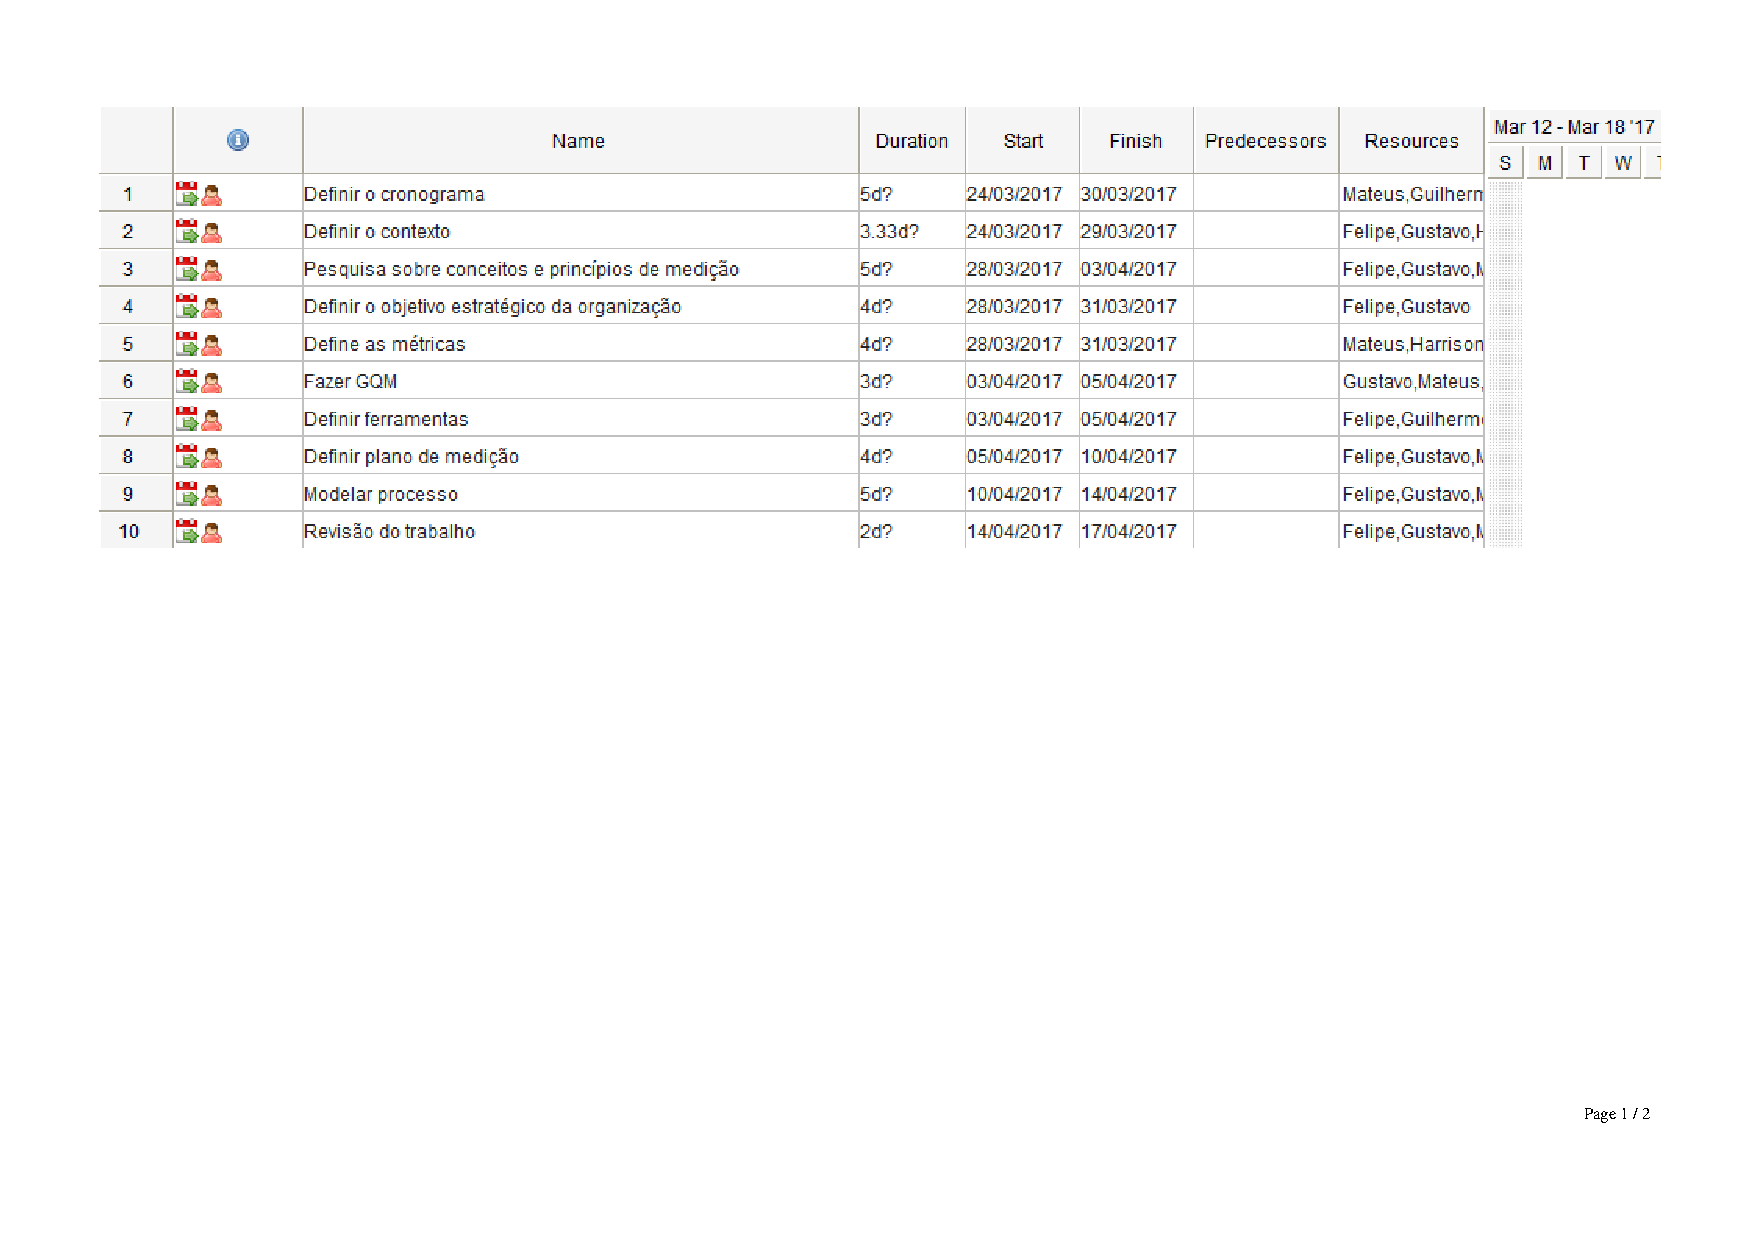
\includegraphics [scale=0.4]{figuras/processo/cronograma}
		\caption{Cronograma utilizado pela equipe}
		content...
	\end{figure}